\chapter{Experiments and Analysis}\label{chap:exp_and_analysis}

% \sectionoutline{i'm thinking of a methods/analysis/results structure like this:
% details on the scaling issues with simulating quantum systems, how they explode unless we find some smart solutions (hint hint stabilizer formalism)

% this motivates beginning by a proof of concept experiment with the smallest codes, where i touch upon the 5 and 7 qubit codes and their properties (maybe i don't really introduce them in the theory section at all, leave their formal descriptions as an appendix?). i explain these experiments however far they get with memory limitations etc

% moving on to why the stabilizer formalism is a helpful tool that lets us do more classically because we can store a state essentially “in terms of its stabilizers” (right?)

% introducing the software package panQEC and some details on how it works internally that support this “easy to compute with stabilizers” argument

% then we show the quantum memory simualtion results with the BB code and surface code.
% now we get into the part i havent really done but i think should be possible: i know panQEC can identify X and Z logicals so it would be interesting to run the simulations again with those applied perhaps, maybe even a hadamard? 

% then we make a similar plot of the logical operators over time

% then we move on to T gates in earnest and CCZ factories and how this is outside the scope of the stabilizer formalism so panQEC probably can't really help us, and then i can show some attempts to code this up on individual logical qubits (not in the grover circuit)}

\section{General Limitations when Simulating Quantum Systems}\label{chap:simulation_limitations}
In order to design and develop the technology necessary to begin implementing new error-correcting architectures, it is typically helpful to simulate how the components might work. In particular, a natural starting point for assessing the resource costs of a fault-tolerant implementation of Grover's algorithm is to simulate the physical qubit setup it would require. However, simulating the full fault-tolerant system with an error-correcting code of our choice turns out to be nearly impossible, even for the smallest nontrivial case of Grover's algorithm with only two input qubits.

To understand why this is so problematic, recall the expression for the unitary matrix defining an arbitrary quantum circuit with $n$ input qubits:
\[U \in \mathbb{C}^{2^n \times 2^n}.\]
Given a gate set, we obtain $U$ by \emph{lifting} the individual gate matrices to the appropriate dimension $2^n \times 2^n$ and multiplying them in the right order. Specifically, in a quantum circuit, lifting a single-qubit gate $G \in \mathbb{C}^{2 \times 2}$ acting on qubit $k$ of an $n$-qubit system means constructing the corresponding $2^n \times 2^n$ unitary
\[
\tilde{G} = \mathbb{I}_2 \otimes \cdots \otimes G \otimes \cdots \otimes \mathbb{I}_2,
\]
where $G$ appears in the $k$-th tensor factor. This approach preserves the mathematical structure of the full state at all times when applying a gate to only a few of the qubits, but it comes at a cost. The exponential scaling when $n$ grows as we add qubits to the system means that we quickly face extremely large matrices when simulating anything beyond minimal examples or the logical abstractions of algorithms. This is bad news for us, as adding the error-correction architectures we are primarily interested in will prevent us from being able to simulate the circuit.

For instance, the smallest possible surface code is displayed in \cref{fig:smallest_surface_code}. \begin{figure}[tb]
    \centering
    
\includegraphics[scale=0.5]{The-smallest-possible-surface-code-consisting-of-9-data-qubits-The-indicated-8.png}
    \caption{Via \textcite{smallestsurfacecode}: ``The smallest possible surface code, consisting of nine data qubits. The indicated eight stabilizers could, in principle, be measured sequentially by a single additional qubit, or measured in parallel by an additional eight qubits.'' Note that in this visualization of the surface code, the grid is rotated 45° compared to the previous representation; the data qubits are the nine white circles instead of on the grid lines, and the ancillary check qubits belonging to each stabilizer are not shown. Each stabilizer measures the four (or two) qubits located at its corners.}\label{fig:smallest_surface_code}
\end{figure}
It requires at least ten qubits, provided we reuse a single ancillary qubit for measurement rather than using eight individual ones for each of the stabilizers. Each gate we would need in a simulation of Grover's with two logical qubits would be a $2^{20} \times 2^{20}$ matrix to account for the no fewer than 20 qubits in the system. A single $2^{20} \times 2^{20}$ complex matrix has $2^{40} \approx 1.1 \times 10^{12}$ entries. Storing each entry as a 64-bit (8-byte) double-precision complex number (i.e.\ two 64-bit floats for the real and imaginary parts) therefore requires
\[
    2^{40} \times 16\ \text{bytes} = 2^{44}\ \text{bytes} \approx 17.6\ \text{TB}
\]
of memory per matrix. In practice, we rarely need to store the full unitary $U$ explicitly; it suffices to track the state vector $\ket{\psi} \in \mathbb{C}^{2^n}$ and apply each lifted gate $\tilde{G}$ in sequence. The state vector itself is far more manageable at $2^{20} \times 16\ \text{bytes} = 16\ \text{MB}$, but each product $\tilde{G}\ket{\psi}$ requires an explicit $2^{20} \times 2^{20}$ matrix, which reintroduces the same memory bottleneck. Exploiting the tensor product structure of $\tilde{G}$ allows this to be replaced by a sequence of much smaller operations, and sparse or structured representations can reduce the constant factor, but the fundamental $\mathcal{O}(4^n)$ memory scaling of an $n$-qubit unitary cannot be avoided in general, and 17.6 TB far exceeds the RAM available on any single consumer machine. This estimation also assumes none of the gates necessitate additional ancilla qubits to further drive up this cost, which, as we will see in \cref{sec:t_gate} when we delve into the implementation of the $T$-gate, is not the case.

% \subsection{Choices to Make When Performing Quantum Computations}
% \sectionoutline{this section has been moved from background. should probably be worked into text in other ways.}

% There are a few separate challenges with doing operations on quantum data that we must address in order to reach our goal of a fault-tolerant circuit for Grover's algorithm. Assuming we have made some choice of error correcting code, first, \ding{192} we must choose an appropriate universal gate set. Next, \ding{193} we need to take the operations we want and determine an equivalent calculation using only the gates in our chosen gate set. Finally, we face another problem entirely in taking our chosen gate set to the quantum hardware and \ding{194} figuring out how the circuit we designed will be implemented on the error-correcting patches corresponding to logical qubits. 

% With regards to \ding{192}...

% \sectionoutline{If it becomes at all interesting to explore other options besides the Clifford+T gate set, I will define and discuss them here. Otherwise, I will elaborate a bit and justify my choice of sticking to Clifford+T.}

% As for the next challenge, while \ding{193} is not necessarily easy in isolation, provided we have our operation expressed as a circuit in some other gate set, there fortunately exist tools such as Synthetiq \cite{synthetiq2025} that can do this optimization and search process for us. In our case with Grover's algorithm, the circuit without restricting which gates we can use is well known, and Synthetiq can be used to convert it into whatever other limited gate set we would like.%\textcolor{blue}{Additionally, the Grover circuit is quite small in the case we are simulating, so it may be fine to just do this manually, or not at all. We should bear in mind the hardware-aware approach though to avoid doing calculations that cancel.}

% In many ways, the trouble with running Grover's algorithm on a quantum machine boils down to \ding{194}. While certain logical operators are known or can be identified by the software tools, others might pose more of a challenge. 

% As highlighted earlier in \cref{chap:grovers_explanation}, the gates we need to perform the full circuit for Grover's algorithm are $H$, $Z_f$ and $Z_{\text{OR}}$. Of these, $H$ is largely considered computationally easy, taking our standard $X$ and $Z$ corrections and swapping them, since $H$ maps $\ket{0}$ to $\ket{+}$, $\ket{1}$ to $\ket{-}$, and vice versa, leaving us in the realm of the computationally easy Clifford gates. 

% The phase query gates $Z_f$ and $Z_{\text{OR}}$ are more problematic, however, and will require the computationally hard T-gates.

\subsection{Proof-of-concept Experiments with Smaller Codes}\label{sec:smaller_code_experiments}
The memory requirements we have now established make a direct simulation of Grover's algorithm on the surface code infeasible even in its smallest instance, so instead we consider alternative codes with lower qubit overhead.

Fault-tolerant physical implementations of Grover's algorithm are only now beginning to be realized \cite{Butt2026}, and a detailed exploration of how they might look at larger scales remains an open and timely problem. The experiments in this section serve two purposes. First, they establish that the logical structure of Grover's algorithm functions correctly under continuous error correction, and second, they demonstrate the classical simulation barrier that motivates the stabilizer-based computational methods used throughout the remainder of the thesis. Two smaller error correcting codes were selected for this purpose: the \emph{5-qubit code} and the \emph{7-qubit Steane code}, both of which are defined and described in more detail in \cref{app:smaller_codes}.

The 5-qubit code is the smallest quantum error correcting code capable of correcting any single-qubit error \cite{Nielsen_Chuang_2010}, making it a natural starting point. Both codes functioned as stable quantum memory under the same procedure: encoding a logical codeword, injecting a single-qubit Pauli error, measuring the syndrome and applying the corresponding correction from a lookup table. All 30 test cases for the 5-qubit code ($X$, $Y$, and $Z$ errors on each of the five physical qubits, applied to both $\ket{0_L}$ and $\ket{1_L}$) were recovered correctly, which was confirmed by computing the \emph{fidelity}, given by $|\bra{\psi_L} \ket {\psi_{\text{corrected}}}|^2$. It can be interpreted as a measure of overlap between the corrected and original states, equal to 1 when they are identical, which is what we found across all test cases. However, the 5-qubit code turns out to be a poor candidate for computation. Clifford gates are not transversal in it, meaning fault-tolerant logical operations become a challenge.

\subsubsection{Simulating Toy Version of Grover's Algorithm}\label{subsec:toyversion}
Thus, we move on to considering the 7-qubit Steane code. Unlike in the 5-qubit code, Clifford gates are transversal in the 7-qubit code, making it a common choice in quantum error correction research today. We can verify its error correction capability in the same fashion as the 5-qubit code, this time implemented using IBM's quantum simulator package \texttt{Qiskit} \cite{qiskit2024}, rather than being coded from scratch.

Once the memory aspect worked as intended, the algorithm itself could be implemented. The logical Hadamard is $H_L = H^{\otimes 7}$, valid because the Steane code is \emph{self-dual}: The same parity-check matrix governs both $X$- and $Z$-type stabilizers, so $H^{\otimes 7}$ exchanges them symmetrically. The logical $X$ is the transversal $X_L = X^{\otimes 7}$, mapping $\ket{0_L}$ to $\ket{1_L}$. A logical controlled-$Z$ between two code blocks is implemented by applying a physical $CZ$ between each pair of corresponding qubits across the blocks.%\supervisors{More explanation required here?}

The oracle and diffusion operators are then built entirely from these three building blocks. Notably, this gate set contains no $T$-gates. With only two logical qubits, the oracle reduces to a single controlled-$Z$, since $CZ$ naturally applies a phase flip of $-1$ exactly when both qubits are $\ket{1}$, which is all a two-element oracle requires. In a cryptographically relevant implementation, the oracle would be replaced by the full AES circuit, whose AND gates decompose into Toffoli gates under the Clifford$+T$ gate set. This is where the $T$ gates enter, reintroducing the overhead that dominates Jaques' resource estimates. The experiment here is therefore a proof-of-concept for the logical structure of fault-tolerant Grover's algorithm, with the computational core of the oracle deliberately kept simple. As such, the target state is explicitly encoded into the oracle circuit, which would not be the case in a real application. In practice, the oracle is a fixed circuit evaluating some function $f$, which recognizes solutions without prior knowledge of what they are.

\begin{quote}
\textbf{Procedure: Grover's algorithm on two Steane-encoded logical qubits}
\begin{enumerate}
    \item \textbf{Encode:} prepare $\ket{0_L}$ for both logical qubits using the
          Steane encoding circuit (14 physical qubits total)
    \item \textbf{Superpose:} apply $H_L = H^{\otimes 7}$ to both blocks
    \item \textbf{Oracle} (applied once, since
          $\lfloor\tfrac{\pi}{4}\sqrt{4}\rfloor = 1$):
    \begin{enumerate}
        \item For each block $i$: if $t[i]=\texttt{0}$, apply $X_L = X^{\otimes 7}$
              \hfill\emph{(flip 0-target bits to 1)}
        \item Apply transversal $CZ_L$ between corresponding qubits of both blocks
        \item Undo the flips from step (a)
    \end{enumerate}
    \item \textbf{Diffusion:} apply $H_L,\; X_L,\; CZ_L,\; X_L,\; H_L$ to both
          blocks
    \item \textbf{Measure:} compute the parity of all 7 physical qubits in each block
          via a single ancilla qubit
\end{enumerate}
\end{quote}

After each step of the algorithm, errors are injected, stabilizers are measured and Pauli corrections applied before the next layer is executed. The error model used is the \emph{depolarizing noise model} \cite{Nielsen_Chuang_2010}, which applies a random Pauli error to a qubit after each gate with some fixed probability $p$, independent of the gate or the state of the qubit. 
The error probabilities $p_1 = 0.001$ for single-qubit gates and $p_2 = 0.01$ for two-qubit gates were selected to reflect the typical performance gap between one- and two-qubit operations on current superconducting hardware, where two-qubit gate fidelities are consistently an order of magnitude worse than single-qubit ones \cite{Li_2023}. These values are representative of near-term device capabilities and place the simulation in a regime where error correction has meaningful but not overwhelming work to do: low enough that the code is operating below its threshold, but high enough that logical errors remain visible on the scale of the experiment. The idle error probability $p_{\text{idle}} = 10^{-5}$ models decoherence on qubits that are not actively participating in a gate layer. 
This is set conservatively low relative to $p_1$ and $p_2$ because idle errors accumulate on a different, slower timescale than gate errors in most hardware platforms~\cite{Li_2023}, and the primary purpose of this experiment is to characterize the impact of gate-level noise rather than memory-level decoherence.

\begin{figure}[tb!]
\centering

\includegraphics[width=\textwidth]{steane_grovers_histogram.pdf}
\caption{Measurement outcome distributions for Grover's algorithm on two Steane $[\![7,1,3]\!]$-encoded logical qubits (1,024 shots each) under depolarizing noise ($p_1 = 0.001$, $p_2 = 0.01$) and the probability of idle qubits being corrupted $p_{\text{idle}} = 10^{-5}$. Error correction is applied continuously throughout the circuit. Each panel targets one of the four logical basis states, identifying the correct state with probability $\approx 0.6$ after a single Grover iteration.}\label{fig:steane_grovers_histogram}
\end{figure}

\Cref{fig:steane_grovers_histogram} shows the outcome distributions for all four target states at 1,024 shots each under this noise model. The correct state is found with probability $\approx 0.6$ after a single iteration. While not a stellar result, it is still clearly an improvement over the the uniform distribution that would result from a completely failed computation. The outcome distributions also match theoretical expectations in that the bitwise complement of the target (the state requiring simultaneous logical errors on both qubits) is consistently the least likely non-target outcome. Outcomes requiring only a single logical failure occur with probability scaling as $p$, while reaching the complement requires two independent logical failures and therefore scales as $p^2$. With $p \ll 1$, the complement is suppressed by an additional factor of $p$ relative to the single-flip outcomes.

It is worth noting that even this simplified experiment of a Clifford-only circuit with no $T$-gates could not be run on a general-purpose statevector simulator without exorbitant memory cost. The circuit uses 28 qubits in total: 14 data qubits across the two logical blocks, 12 error correction ancilla qubits, and two readout ancilla qubits. Simulating this classically as a full statevector requires storing $2^{28}$ complex amplitudes, which at double precision amounts to exactly 4\,GB. This is already at the limit of what a typical consumer machine can hold for a single process, before accounting for the working memory the simulator additionally requires. The simulation is only tractable here because the \texttt{AerSimulator} in \texttt{Qiskit} exploits aspects of the stabilizer code structure introduced in \cref{sec:toriccode} to sidestep the full vector simulation entirely. Previously, we considered stabilizers a tool for QEC, but as we will see, they turn out to be useful as a means of efficient classical simulation as well.

\section{Utilizing Stabilizer Formalism as a Computational Tool}\label{sec:stabilizers_in_computation}
The exponential scaling of full unitary simulation, as described in \cref{chap:simulation_limitations}, presents a fundamental barrier to classical simulation of large quantum circuits. In certain codes, however, we can at least partially circumvent the issue: For an $n$-qubit system, rather than storing and manipulating the full $2^n \times 2^n$ unitary, or even the state vector of $2^n$ complex amplitudes, a stabilizer state can be represented compactly by a set of $n$ independent commuting Pauli operators $\{g_1, \ldots, g_n\}$ called \emph{generators}. This uniquely specifies a state $\ket{\psi}$, which is the one joint $+1$ eigenstate of all $g_i$ simultaneously. Thus, to recover the state vector from the generators, one simply asks which state satisfies $g_i\ket{\psi} = +\ket{\psi}$ for all $i$. To further illustrate how the stabilizer representation lets us recover the corresponding state vector uniquely, we will step through a small example.

\begin{center}
    \begin{tikzpicture}
    \node [mybox] (box){%
        \begin{minipage}{0.85\textwidth}
            Consider the 3-qubit bit-flip code, with stabilizers $g_1 = ZZI$ and $g_2 = IZZ$, and logical operators $\bar{X} = XXX$, $\bar{Z} = ZZZ$. The generators alone define the codespace, spanned by $\ket{\bar{0}} = \ket{000}$ and $\ket{\bar{1}} = \ket{111}$, but do not yet specify which logical state we are in. To define a specific state, we augment the generator list with a logical operator. If we add $\bar{Z} = ZZZ$ as a third stabilizer, the unique joint $+1$ eigenstate of all three is $\ket{000} = \ket{\bar{0}}$, since we see that $ZZZ\ket{111} = -\ket{111}$, ruling out $\ket{111} = \ket{\bar{1}}$ as it is not a +1 eigenstate of the set. If we add $\bar{X} = XXX$ instead, the unique joint $+1$ eigenstate becomes $\frac{1}{\sqrt{2}}(\ket{000} + \ket{111}) = \ket{\bar{+}}$. In each case, the full state vector is recoverable from the generator list alone, with no ambiguity.
        \end{minipage}
    };
    \node[fancytitle, right=10pt] at (box.north west) {Example: Recovering a state vector from the stabilizer representation};
    \end{tikzpicture}%
\end{center}

The storage advantage is now clear: Each generator $g_i$ is a tensor product of $n$ single-qubit Paulis, requiring only $\mathcal{O}(n)$ bits to store. Since we know the number of stabilizers we need is also on the order of $n$, the full generator list needs only $\mathcal{O}(n^2)$ bits, compared to $\mathcal{O}(2^n)$ complex numbers for the state vector. 

We also have computational shortcuts when working with Clifford gates, which we recall from \cref{subsec:cliffordplust} are the gates that map Pauli operators to Pauli operators under conjugation. If we have a stabilizer state $\ket{\psi}$ with generators $\{g_1, \ldots, g_n\}$, we can apply a Clifford gate $C$ to obtain a new state $C\ket{\psi}$. Rather than computing the full matrix product $C\ket{\psi}$ in a $2^n$-dimensional space, we can take advantage of the stabilizer formalism and the fact that the generators uniquely determine the state to calculate the effect of $C$ based on what happens to the generators. We want a new set of operators $g_i'$ such that $g_i'(C\ket{\psi}) = C\ket{\psi}$, which the map $ g_i \;\mapsto\; Cg_iC^\dagger$ achieves. We can verify that generators $g_i' = Cg_iC^\dagger$ defined in this way do indeed stabilize our updated state $C\ket{\psi}$, since it holds that
\[g_i'C\ket{\psi} = Cg_iC^\dagger \cdot C\ket{\psi} = Cg_i\ket{\psi} = C\ket{\psi}.\]
This stabilizer update rule holds for any unitary matrix, but working with Clifford gates unlocks the advantage of ensuring $Cg_iC^\dagger$ is always another valid Pauli string, preserving the compact $\mathcal{O}(n)$-bit-per-generator storage throughout the entire computation. If conjugation by $C$ could produce arbitrary matrices, we would be back to storing exponentially large objects and the efficiency gain would be lost.

To see the mechanics of the update rule, consider applying $H$ to $\ket{0}$, stabilized by $g = Z$. We can simply update the stabilizer $HZH^\dagger = X$ and read off that the new state is stabilized by $X$, meaning it is the state $\ket{+}$. No matrix multiplication of a state vector is needed; the state update is captured in its entirety by relabeling one Pauli letter. In general, since a Clifford gate touches at most two qubits at a time (with the two-qubit gate $CNOT$ being the only fundamental Clifford gate acting on more than one qubit), updating one generator costs $\mathcal{O}(1)$, relabeling at most two Pauli letters according to a fixed lookup table. Updating all $n$ generators therefore costs $\mathcal{O}(n)$ in total, compared to the $\mathcal{O}(2^n)$ cost of full state vector simulation. This is the main result of the Gottesman-Knill theorem \cite{gottesman1998heisenbergrepresentationquantumcomputers}: Any circuit composed entirely of Clifford gates can be simulated efficiently on a classical computer in the stabilizer representation. This is exactly the trick the \texttt{AerSimulator} from \texttt{Qiskit} utilized to simulate our 28-qubit system in \cref{subsec:toyversion} by representing the quantum state as a set of stabilizers, rather than a full state vector.

\subsection{Simulating Stable Quantum Memory with PanQEC}\label{subsec:panqec_memory}
% \supervisorsinline{I used toric code throughout experiments (periodic boundary conditions and 2 logical qubits encoded instead of 1). I can use the surface code isntead which is maybe a little more realistic but then the scale of the surface code may be hard to simulate and decode properly.}
A natural place to begin our investigation into the merit of the BB code is with quantum memory. To do so, the QEC simulation and visualization package \texttt{PanQEC} \cite{panqec2021} was used to visualize the geometry of several error correcting codes and to extract their logical operators. It stores stabilizer codes internally in \emph{binary symplectic format}, in which each Pauli operator on $n$ qubits is represented as a binary vector $v = (v_X \mid v_Z) \in \mathbb{F}_2^{2n}$, the vector space of binary strings of length $2n$. Here, the first $n$ bits indicate which qubits carry an $X$ factor and the last $n$ indicate which carry a $Z$ factor. A full stabilizer group with $m$ generators is then stored as an $m \times 2n$ binary matrix, replacing what would otherwise require tracking $m$ dense $2^n \times 2^n$ matrices. This yields a significant reduction in memory overhead and makes operations such as checking commutativity straightforward via the symplectic inner product.

As a baseline and to verify the correctness of our \texttt{PanQEC} implementation, we do a quantum memory threshold simulation, shown in \cref{fig:gross_vs_toric}, where we compare the gross code to the surface code with identical logical qubit counts, in order to say something meaningful about the architectural trade-offs relevant to Jaques' assumptions. The depolarizing error model was kept constant across all experiments. In addition, all experiments use the \emph{Belief Propagation with Localized Statistics Decoding} (BP+LSD) decoder to determine the corrections to make based on the syndrome of the error \cite{Hillmann_2025}. We compare logical error rate as a function of physical error rate under Monte Carlo sampling. 

\begin{figure}[hb!]
    \centering
    
\includegraphics[scale=0.8]{gross_vs_toric.pdf}
    \caption{Quantum memory simulation results comparing the BB code (orange) against toric code implementations at identical logical qubit counts (light blue), as well as matching code distance (dark blue). Logical error rate is plotted as a function of physical error rate under Monte Carlo sampling.}\label{fig:gross_vs_toric}
\end{figure}

\subsubsection{Results}
At matched logical qubit count ($k = 12$), the gross code reaches a lower logical error rate at equivalent physical error rates, consistent with its more favorable qubit overhead ratio: The surface code requires $n = 192$ physical qubits to encode 12 logical qubits at distance $d = 4$, while the gross code achieves the same $k$ at $d = 12$ using only $n = 144$. At matched $k$ and $d$, we now see that the surface code is able to correct roughly the same number of errors as the gross code, which aligns with the theory given the equal code distance. However, there is now a huge disparity in the number of physical qubits required for the surface code to do this correction, as it requires $n = 1728$ physical qubits for equivalent error protection, a factor of twelve more than the gross code. This confirms the memory-level improvement that motivates our choice of BB code as an alternative architecture, and identifies the physical error rate at which the gross code operates reliably as $p \approx 0.10$ in this experimental setup. %All subsequent experiments are conducted with this error rate.

\subsection{Simulating Transversal Logical Operators with PanQEC}\label{sec:panqec_gates}
Having established that the BB code offers an advantage over the surface code at the level of quantum memory, the natural next question is whether this advantage persists once we require the code to support logical computation. Jaques' argument, as discussed in \cref{sec:jaques}, identifies the cost of fault-tolerant gate implementation (specifically, the T-gate) as the dominant resource bottleneck, not memory overhead. The memory result therefore motivates but does not resolve the question of whether BB codes meaningfully improve the outlook for Grover's algorithm in practice. To begin probing this, we return to \texttt{PanQEC}, which has functionality for determining logical operators of various types, identifying which physical qubits we would have to modify to correspond to a gate application on the logical qubits. We call this set of qubits the \emph{gate support} of the logical gate, which has a \emph{weight} equal to the number of qubits in the set $w$.

The experiment proceeds as follows. For both the BB code and the toric surface code, both instantiated at $n = 98$ physical qubits ($L_x = L_y = 7$), the \texttt{PanQEC} logical operator matrices $\mathbf{l}_X$ and $\mathbf{l}_Z$ are extracted directly from the %\texttt{bposd} CSS 
code object. Each row of $\mathbf{l}_X$ is a binary vector of length $n$ identifying the physical qubits on which a representative $\bar{X}$ operator acts. The minimum-weight row is selected as the gate support, which we interpret as the most qubit-efficient realization of the logical gate.

To simulate gate noise, $X$-errors are injected independently on each gate-support qubit with probability $p$, modeling the scenario where each physical gate operation fails with that probability. No errors are placed on the remaining $n - w$ qubits, reflecting the principle that each gate application is an independent opportunity for error \cite{Nielsen_Chuang_2010}. Since errors are injected only on the support qubits, we isolate the effect of gate noise so any logical failure is directly attributable to the gate, not to background memory errors. 
This is a narrower question than the full fault-tolerance threshold of \textcite{Bravyi2024}, which models circuit-level noise across every operation in the syndrome measurement cycle, but it is the relevant one here: The BB code's heavier gate support means errors are concentrated on more qubits per gate application; it is not obvious a priori that its higher distance compensates for this.
The BP-LSD decoder determines corrections, and the residual error is checked against $\mathbf{l}_Z$ to assert logical failure. This will only occur when the decoder is fooled, which happens when the error pattern, combined with whatever correction the decoder applies, leaves a residual that is a logical operator $\bar{X}$. Since $\bar{X}$ commutes with all stabilizers by definition, it produces no syndrome and passes through the decoder undetected, silently flipping the logical state.

$10^6$ Monte Carlo trials are run per error rate. A distance-$d$ code corrects any error pattern of weight up to $\lfloor \frac{d-1}{2} \rfloor$, so the smallest uncorrectable pattern has weight $d_e = \lfloor \frac{d-1}{2} \rfloor$, which we call the \emph{error dimension}~\cite{Fowler_2012}. Since each independent error occurs with probability $p$, the leading-order logical failure probability scales as $p_L \propto p^{d_e}$ in the low-$p$ region. With $10^6$ trials per point, the smallest resolvable failure probability is on the order of $10^{-6}$, where only a few failures are observed. The lowest measured points therefore carry large relative uncertainty and several fall at or near this resolution floor. The power-law fit is used to extrapolate below the floor into the low-$p$ region where direct Monte Carlo cannot resolve individual logical failures.

\begin{figure}[h!]
    \centering
    
\includegraphics[width=\linewidth]{gate_support_visualization.pdf}
    \caption{Physical qubits activated during a transversal $\bar{X}$ gate (colored stars) versus idle qubits (gray), for the BB code $[[98, 6, 12]]$ (left, yellow) and the toric surface code $[[98, 2, 7]]$ (right, blue), both at $n = 98$ physical qubits. %The BB code gate support has weight $w = 18$; the toric code gate support has weight $w = 7$.
    }\label{fig:gate_support}
\end{figure}

\subsubsection{Results}

\Cref{fig:gate_support} displays the gate support of the minimum-weight $\bar{X}$ representative the decoder identified on the physical lattice for each code. For the toric surface code $[[98, 2, 7]]$, the gate support weight equals the code distance ($w = d = 7$): The gate support is exactly the minimum-weight logical $X$ representative, so the shortest path implementing the logical gate is also the easiest path for the decoder to confuse with a logical error. For the $[[98, 6, 12]]$ BB code \cite{eberhardt2024logicaloperatorsfoldtransversalgates}, the decoder returns $\bar{X}$ representatives of weight 18, which is the gate support used in the simulation. These are not guaranteed to be the minimum-weight representatives of their logical class, which is an NP-hard problem in general, but they are valid logical operators and represent a concrete gate implementation.

\begin{figure}[b!]
    \centering
    
\includegraphics[width=\linewidth]{gate_error_vs_memory.pdf}
    \caption{Logical $\bar{X}$ failure probability (log scale) as a function of per-qubit gate error rate $p$, for the BB code $[[98, 6, 12]]$ (yellow, $w = 18$) and toric surface code $[[98, 2, 7]]$ (blue, $w = 7$), both at $n = 98$ physical qubits. Dashed lines show a power-law fit $p_L \propto p^{d_e}$ to the observed data, extrapolated into the low-$p$ regime where $10^6$ Monte Carlo trials are insufficient to resolve individual logical failures. The exponent is the error dimension $d_e = \lfloor \frac{d-1}{2} \rfloor$~\cite{Fowler_2012}.%The dotted line marks the crossover at $p \approx 0.30$; current superconducting hardware operates in the shaded region well to the left.
    }\label{fig:gate_error}
\end{figure}

\Cref{fig:gate_error} shows the logical error rate of the codes after injecting errors on the individual qubits in the gate support, followed by the decoder's corrections. Results are plotted on a logarithmic scale to resolve the small failure probabilities at realistic error rates. Through repeated trials across a wide range of physical error rates, it was determined that a crossover occurs near $p \approx 0.30$, above which the surface code becomes more tolerant. This crossover is a consequence of two competing effects: A larger gate support creates more potential error sites (disadvantaging the BB code), while higher code distance allows more errors to be corrected (favoring it). However, since current superconducting two-qubit gate error rates are typically below 1\%~\cite{advancementsinquantumcomputing,jaques2024ches_presentation}, the physically relevant regime lies well to the left of this crossover, and \cref{fig:gate_error} is therefore plotted only up to $p = 0.10$ to focus on this region. 

We see that throughout this regime, the BB code $[[98, 6, 12]]$ achieves lower logical failure probability than the toric code $[[98, 2, 7]]$, despite its gate support being about 2.6 times larger ($w = 18$ versus $w = 7$). The code's higher distance ($d = 12$ versus $d = 7$) more than compensates for the larger number of gate-error sites. Furthermore, provided the operators we identified are in fact the minimum-weight operators, the heavier gate support of the BB code also means that the probability of enough simultaneous errors to cause a logical failure scales as a higher power of $p$, making undetected logical failure exponentially less likely at realistic error rates.

% \supervisorsinline{i thouhgt of some limitations of this experiment as is. do i talk about them here?

% 1. Only X errors. Testing only X against $\mathbf{l}_Z$ is half the picture. worth changing? 

% 2. The gate support might not be optimal. $w=18$ for the BB code may not be minimum-weight, so this might be a suboptimal implementation, which undersells it.

% 3. Doesn't really address Jaques' actual concern, the whole thesis motivation is T-gate cost, and this experiment tests Clifford gates. It's just a stepping stone on the way}


\section{The Trouble with the \texorpdfstring{$T$}{T}-gate}\label{sec:t_gate}
%\todo[inline]{in this section, we discuss what resources we physically need (also the time it takes) to implement T gates. we do not dicuss the amount of t gates necessarily, that's part of the grande finale argument in 3.4. any discussion of that should be moved out of this section and is probably repeated in section 3.4.}

As established in \cref{subsec:cliffordplust}, the $T$-gate's incompatibility with the Pauli group under conjugation means it cannot be implemented by any manipulation of the stabilizer structure alone. This has a direct consequence for classical simulation: The moment a $T$-gate is introduced into a circuit, the stabilizer update rule $g_i \mapsto Cg_iC^\dagger$ no longer produces a valid Pauli string, the compact $\mathcal{O}(n^2)$ stabilizer representation breaks down, and we must fall back to full state vector simulation at exponential cost. This is why the efficient classical simulation guaranteed by the Gottesman-Knill theorem for Clifford circuits, discussed in \cref{sec:stabilizers_in_computation}, does not extend to circuits containing $T$-gates.

The standard route to a fault-tolerant T-gate is \emph{magic state distillation} (MSD) \cite{Bravyi_2005}. The central idea is to separate the non-Clifford content of a computation from its execution: rather than applying a T-gate directly to a data qubit at runtime, one instead prepares a state $\ket{T} = T\ket{+}$ in advance using only noisy physical operations, which we call a \emph{magic state}. Then, through a method known as \emph{gate teleportation}, the magic state is consumed, and we effectively transfer it from the ancilla qubit to a data qubit by entangling the two and then measuring the ancilla \cite{Nielsen_Chuang_2010}. In short, this is a way to apply a non-Clifford (non-transversal) gate to a data qubit without direct application, at the cost of measuring (and thus destroying) the state prepared in the ancilla. All the necessary non-Clifford action is concentrated into preparing the magic state in advance; the rest of the computation then proceeds using only Clifford gates and measurements.

The difficulty is that magic states prepared directly from noisy physical operations are themselves noisy, and consuming a low-fidelity magic state introduces errors into the computation. MSD resolves this by taking multiple noisy copies of $\ket{T}$ and combining them through a carefully designed Clifford circuit to produce a smaller number of copies with substantially higher fidelity. The dominant protocol for distillation of $\ket{T}$ is the 15-to-1 scheme \cite{Bravyi_2005}. In it, 15 noisy input magic states are consumed to produce a single output state whose error rate scales as the cube of the input error rate, providing cubic suppression at the cost of a fifteen-fold resource overhead. The physical unit that executes this protocol is called a \emph{magic state factory}, and in large-scale fault-tolerant architectures, it is common for the majority of physical qubits to be devoted to running factories rather than to the logical computation itself \cite{Xu_2026}. This distillation can also be applied iteratively. Letting $p_{\text{input}}$ denote the error rate of the noisy input magic states, feeding the output of one round as input to the next yields error rates scaling as $p_{\text{input}}^{3^L}$ after $L$ levels, at a resource cost of $15^L$ input states per output~\cite{Bravyi_2005}.

Recent work by Xu et al.\ \cite{Xu_2026} designs concrete MSD factories tailored to the BB architecture, providing direct resource comparisons against surface code factories. At a physical error rate of $p_{\text{phys}} = 10^{-3}$, their gross-code-based factories require substantially fewer physical qubits than a surface code factory achieving the same target output error rate. Crucially, however, the total space-time volume of magic state production (the product of physical qubits and syndrome extraction cycles, and a more complete measure of total resource cost) is comparable between the two architectures. The BB code does not reduce the time required to produce a single magic state, but rather it achieves the same output quality at a smaller physical footprint, with the cycle cost remaining broadly similar. For a fixed hardware budget, this smaller footprint in principle allows more factories to run in parallel, potentially improving $T$-gate throughput, but each factory still takes a comparable number of syndrome cycles per magic state produced. They further identify BB code factories as particularly well-suited as the second stage in a two-level distillation pipeline, following an initial step performed on a surface code.

% Crucially, this protocol is code-agnostic at the logical level\todo{source}, meaning the same 15:1 logical circuit is used regardless of which physical code is chosen to encode each magic state patch.  The choice of code affects only how many physical qubits each logical patch requires and how many syndrome measurement cycles are needed per factory run.

% \subsection{Implemention}
% \todo[inline]{Show the minimal attempt (and explain where it breaks down if the experiment can't be successfully completed)}

% \todo[inline]{Add pseudocode for T-gate on individual error corrected qubits, not in a full circuit.}

% PSEUDOCODE GOES HERE!

\section{Assessing the Quantum Threat}\label{sec:quantum_threat}
In \cref{sec:jaques}, we reviewed Jaques' argument against the quantum threat to AES, which rests on three distinct pillars: First, the high physical-to-logical qubit ratio obscures the true scale of engineering required to construct working quantum computers that can run Grover's algorithm. Second, fault-tolerant gates carry a significant computational cost. Third, Grover's algorithm parallelizes badly. Together, these factors make the circuit conceptually more complex, and increase both its resource requirements and total runtime. The specifics of Grover's poor parallelism (which is unrelated to the choice of error-correcting code) were covered in \cref{sec:grovers_explanation}, and the experiments in \cref{sec:stabilizers_in_computation,sec:t_gate} were designed to probe the other pillars of the argument under the assumption of the BB code instead of the surface code. %We were able to experimentally verify that the BB code will most likely lower the requirement of physical qubits necessary for stable quantum memory. 
However, in this section, we will argue that even with the improvements afforded by the BB code, constructing stable physical qubits is not the true limitation, as Jaques also points out.

\vspace{1cm}

The memory threshold results of \cref{subsec:panqec_memory} show that the BB code is capable of reducing the physical qubit overhead substantially: At matched logical qubit count and code distance, the surface code requires twelve times as many physical qubits as the gross code. The gate noise results of \cref{sec:panqec_gates} indicate that this advantage persists under gate-level error injection, but more marginally. Therefore, adopting the BB code arguably brings the necessary physical qubit requirements closer to a conceivable scale. The physical-to-logical qubit ratio is not necessarily fixed at 1000:1; under the gross code, it is closer to 12:1 at equivalent error protection.
%\todo[inline]{I want to make clear that a circuit design for Grover's for breaking AES has already been proposed, and i am using the numbers form that analysis to show that this cannot happen. The reason we don't see the speedup people are talking about is because that is for the logical circuit, which is way easier. That's the entire point I've been making! We NEED error correction, but introducing error correciton makes things harder than they seem based on the Big O notation logical circuit.}

% The gate count for implementing Grover's algorithm on AES has been an active area of optimization since the original estimates of \textcite{grassl2015applyinggroversalgorithmaes}, who designed a circuit requiring on the order of $2^{86}$ Clifford gates and $2^{80}$ $T$-gates in total across all Grover iterations. The vast majority of these gates are in the AES circuit in the oracle itself \cite{grassl2015applyinggroversalgorithmaes}. These figures are more or less architecture-agnostic, besides the fact that constructing a circuit based on the Clifford$+T$ gate set in the first place is considered a suitable choice for surface codes. Subsequent work has improved the efficiency of the AES oracle circuit: \textcite{cryptoeprint:2019/1146} introduced depth-optimized implementations with substantially reduced per-oracle-call $T$-counts, and more recent work \cite{resourcefficientAES, cryptoeprint} has further reduced both $T$-depth and qubit footprint. However, these optimizations reduce the cost per oracle call by at most a small constant factor, while the number of oracle calls required is fixed entirely by the search space size, at approximately $\lfloor \frac{\pi}{4} \sqrt{2^{128}} \rfloor \approx 2^{63}$ iterations for AES-128, regardless of how efficiently the oracle is implemented. Since the $T$-gates enter only through the oracle, the total $T$-gate count is simply the per-call count multiplied by the number of iterations, and a constant-factor improvement to the former leaves the overall scaling unchanged. We therefore retain the $2^{80}$ figure from \textcite{grassl2015applyinggroversalgorithmaes} as a conservative baseline. This raises the question: since quantum gates are processes rather than physical devices, how much time would these operations require?

The gate count for implementing Grover's algorithm on AES has been an active area of optimization since the original estimates of \textcite{grassl2015applyinggroversalgorithmaes}, who designed a circuit requiring on the order of $2^{86}$ Clifford gates and $2^{86}$ $T$-gates in total across all Grover iterations. The only place where $T$-gates occur is in the oracle, specifically in the S-box step of AES \cite{cryptoeprint:2019/1146}. The gate counts are more or less architecture-agnostic, besides the fact that constructing a circuit based on the Clifford$+T$ gate set in the first place is considered a suitable choice for surface codes. Subsequent work has been able to reduce this figure: \textcite{cryptoeprint:2019/1146} introduced depth-optimized oracle circuits and showed that fewer AES evaluations are required per oracle call, reducing the total $T$-gate count. More recent circuit optimizations \cite{resourcefficientAES, cryptoeprint} pushed the improvements further, placing the current best estimate for the total serial $T$-gate count required for the full Grover circuit at approximately $2^{80}$.

Unlike classical gates, quantum gates are processes rather than physical devices \cite{jaques2024ches_presentation}. This raises the important question of how much time it will take to execute this circuit in full. To make a lower bound estimate, we begin by simplifying our calculation with the assumption that operations corresponding to Clifford gates are essentially free, meaning we can focus on the $2^{80}$ figure for $T$-gate cost. 
Another assumption we make is that individual quantum operations will be at least as slow as current classical operations. By NIST's estimation, current\footnote{as of 2017} classical computing architectures can perform $2^{64}$ operations serially in a decade \cite{NIST2016pqc}. Using their estimate, the naive calculation of the time it will take to perform $2^{80}$ operations is thus:
\[2^{80} = 2^{16+64} = 2^{16} \cdot 2^{64} = 65,536 \cdot 2^{64}.
\]
With $2^{64}$ operations serially per decade, it will take 655,360 years to complete the calculation of the $T$-gates alone. However, this number assumes no parallelism whatsoever, and the $2^{80}$ $T$-gate figure assumes a single machine searching the full $2^{128}$ key space. One might hope, then, that partitioning the key space among $P$ machines reduces the per-machine circuit depth, which turns out to be true: 
% Each machine searches $\frac{2^{128}}{P}$ keys, requiring only $\sqrt{\frac{2^{128}}{P}} = \frac{2^{64}}{\sqrt{P}}$ Grover iterations, and therefore $\frac{2^{80}}{\sqrt{P}}$ $T$-gates per machine. 
Each machine is assigned a partition of $\frac{2^{128}}{P}$ keys, which becomes its effective search space $N' = \frac{2^{128}}{P}$. 

The number of Grover iterations $t'$ required to search this reduced space is determined by
\[
    t' = \left\lfloor \frac{\pi}{4\theta'} \right\rfloor, \qquad
    \theta' = \sin^{-1}\!\left(\sqrt{\frac{1}{N'}}\right)
            \approx \frac{\sqrt{P}}{2^{64}},
\]
giving $t' \approx \frac{2^{64}}{\sqrt{P}}$, a reduction by a factor of $\sqrt{P}$ relative to the single-machine case. Since the $T$-gate cost of each oracle call is fixed, the per-machine $T$-gate count reduces proportionally to $\frac{2^{80}}{\sqrt{P}}$. However, as established in \cref{sec:parallelism_arg}, this relief comes at a cost. The total $T$-gate count across all machines is
$P \cdot \frac{2^{80}}{\sqrt{P}} = \sqrt{P} \cdot 2^{80}$,
which grows with $P$. \Cref{fig:parallelism_tradeoff} shows both quantities as
functions of $P$. 

\begin{figure}[bt!]
    \centering
    
\includegraphics[width=\linewidth]{parallelism_tradeoff.pdf}
        \caption{$T$-gate cost of Grover's algorithm on AES-128 as a function
    of the number of machines $P$, each searching an equal partition of
    the $2^{128}$ key space. The per-machine cost (blue) decreases as
    $2^{80}/\sqrt{P}$, while the total cost across all machines (orange)
    increases as $\sqrt{P} \cdot 2^{80}$. The horizontal line
    marks the 50-year viability threshold of $2^{66.3}$ $T$-gates per
    machine, which would require approximately $2^{27.4}
    \approx 185$ million machines (vertical line). At this point,
    the total $T$-gate count across all machines reaches $2^{93.7}$,
    nearly $2^{14}$ times the naive single-machine estimate of $2^{64}$.}\label{fig:parallelism_tradeoff}
\end{figure}

As a concrete example, suppose we define a viable attack as one in which each machine completes its share of the computation in under 50 years, i.e.\ at most $5 \times 2^{64} \approx 2^{66.3}$ $T$-gate operations per machine. Setting $\frac{2^{80}}{\sqrt{P}} = 2^{66.3}$ and solving for $P$ gives $P = 2^{27.4} \approx 185$ million machines. At this point, the total $T$-gate count across all machines is $\sqrt{P} \cdot 2^{80} = 2^{93.7}$, which is nearly ten billion times the naive quantum estimate of $2^{64}$. Parallelization does not resolve the runtime problem; it can at best translate a time limitation to a question of hardware, but at an inordinately large scale, while substantially worsening the runtime problem in aggregate.

The impact of the BB code on these figures, as established in \cref{sec:t_gate}, is to reduce the physical qubit
cost of a 15-to-1 magic state factory by roughly a factor of 12
\cite{Xu_2026}. However, it does so by increasing the number of syndrome cycles per factory run, leaving the space-time volume of magic state production comparable to the surface code equivalent. The qubit saving translates in principle to more parallel factories under a fixed hardware budget, but this does not reduce the number of $T$-gates the circuit requires, nor the time each factory takes to produce a single magic state. Thus, there is no evidence of a reduction in the resources required to construct the machinery we would need at this enormous scale. A constant multiplicative improvement to the physical qubit cost does not change the exponential scaling of the total resource requirement.

A natural question is whether code switching could circumvent this limitation. 
In fact, the 15-to-1 MSD scheme already exploits exactly this idea by using 15-qubit Reed-Muller code, in which the $T$-gate is transversal, in order to create magic states~\cite{Bravyi_2005}. This is not a cheap operation. The factory is resource-intensive, and as established in \cref{sec:t_gate}, the majority of physical qubits in a large-scale fault-tolerant architecture are devoted to running these factories rather than to the logical computation itself. More fundamentally, no architectural choice of this kind changes the serial $T$-gate count of $2^{80}$, which is determined entirely by the structure of the AES oracle and the Clifford$+T$ circuit decomposition it requires.

To truly emphasize the infeasibility of this setup, recall also that this lower bound assumes the $2^{86}$ Clifford gates in this circuit design are completely negligible, and that the \emph{hundreds of millions} of quantum machines we require access to all run at the speed of current classical computers. Each of these is already a significant overestimate of near-term capability, and they do not all hold at once. 
As of 2025, the largest quantum processors contain on the order of a few thousand physical qubits \cite{Manetsch_2025}, placing the required scale many orders of magnitude beyond the current state of the art. It is possible that in building the machines we would need to break AES with Grover's algorithm, using the BB code architecture over the surface code architecture could grant a $12\times$ improvement in terms of physical qubits, but there is nothing about using the BB code specifically that addresses the runtime limitation, seeing as it does not reduce the number of $T$-gates we must apply serially.
The prognosis for Grover's algorithm for AES is therefore technically better with something like the gross code---the 185 million machines we would need could possibly be built with 12 times fewer qubits than if we were to use the surface code---but clearly, the engineering gap remains enormous in absolute terms.

This forms the central conclusion of this thesis: Even with the adoption of BB codes, either the computation runs for an astronomically long time, or reducing the runtime to a conceivable scale will have physical architecture requirements that the choice of the error-correcting code cannot address, since the code determines qubit cost per machine, not how many machines we need.
The only way to make any improvement here is to address the estimate of $2^{80}$ $T$-gates applied serially, and whether an error-correcting code with a different native transversal gate set admits a more efficient implementation of the AES oracle. If it can be expressed more efficiently, the $2^{80}$ figure could in principle be reduced not by a constant factor but by a change in the dominant term, which is the only kind of improvement that would materially alter the conclusion reached here. BB codes will not be a good candidate for this use case, since they retain the same Clifford+$T$ logical gate structure as the surface code, with non-transversal $T$-gates handled identically through magic state distillation.

% % For Grover's algorithm to be viable, we need to make other changes besides simply our choice of error-correcting code. While it seems unlikely that we should aim to imrpove our lower bound by increasing the number of operations our computers can perform serially in a decade (seeing as the assumption that quantum computers can perform operations at this speed is already a stretch), it may be possible to further improve the logical circuit design with the Clifford+$T$ gate set in order to bring the $2^{80}$ figure down.\todo{This could be possible, because it is 12 years old afetr all. Also, how does this scale? How much better than $2^{80}$ would we have to do for this to become scary?} 

% % Alternatively, the development of vastly different error correcting architectures that are used with a completely different gate set than Clifford+$T$ will also greatly change the landscape and the lower bound we estimate here. Logical circuit designs would have to be completley remade, as would the methods of implementing the individual nontransversal gates. 

% % All of this is to say that as long as the choice to develop and use BB codes does not also involve instating a different default choice of gate set with a more efficient construction in the BB code, we will most likely not see signicant improvements to the lower bound estimates of Grover's algorithm. 

% % What would need to change? Either we need to design a better logical circuit using Clifford+T to bring the $2^{80}$ number down by a lot, or maybe use a different gateset entirely (which would also require that we remake the logical circuit). Or, if new technology makes it so we can perform more than $2^{64}$ operations in a decade, that will also significantly change things.

% % Main difference with something like the BB code is that physical qubit count becomes less of an issue and the thing about the number of qubits necessary covering the surface of the moon becomes less of an argument against this. 

% % In the first part of his argument, he talks about the fact that we need thousands of logical qubits per physical qubit. BB codes do actually help in this sense, requiring us to build fewer stable qubits.

% % In the next part of his argument, he points out that Grover's has bad parallelization, and this is at the algorithm level so BB codes don't help in this sense.

% % Finally, he talks about 

% % In 2015, \textcite{grassl2015applyinggroversalgorithmaes} found out that we would need on the order of $2^{86}$ Clifford gates and $2^{80}$ T gates to break AES-128. We can consider these processes/time steps. They also say that we would need 2,953 qubits, which is where we get this figure from. 

% % What I'm thinking is that this entire estimate is probaby based on the surface code, and someone has essentially just put in the work to construct this in a diagram and seen that this is what it would take. 

% % All those numbers more or less stay the same in the BB code. So the question is, is implementing a $T$-gate, let alone $2^{80}$ of them, somehow easier/cheaper in the BB code compared to the surface code?

% % From the perspective that we are limited by the number of physical qubits we can build, then yes, BB codes an significantly alter the state of things. But Jaques doesn't think so, because although that is an engineering challenge, the main problem is the time requirements to do $2^{80}$ operations serially.

% % NIST estimates that current classical computing architectures can perform $2^{64}$ operations serially in a decade. The naive calculation is that $2^{80} = 2^{16+64} = 2^{16} \cdot 2^{64} = 65,536 \cdot 2^{64}$, and if we recall that $2^{64}$ operations can be performed serially in a decade, this will take 655,360 years with the $T$-gates alone. However, this number assumes no parallelism whatsoever. 

% % Ideas for parts:

% % A closer look: Do we really need $2^{80}$ $T$-gates? Is the estimate of this from 2016 architecture-agnostic?

% % What gateset could be use instead? What error correcting architectures could we use instead? Is there a future in which qubit quality is high enough that we can get around error correction?

% % Has the technology advanced enough that the $2^{64}$ operations per decade figure has changed? This estimate is from 2017, after all.

% % We will not improve this $2^{64}$ estimate considerably, I don't think.

% % \subsection{T-gate Cost as a Bottleneck}
% % How T-gate count in the Grover circuit translates to physical resource requirements

% % Comparison across codes: surface code vs. BB code overhead per logical T-gate

% % Even with BB code's improved qubit ratio, does the T-gate problem go away?

% % \subsection{Improvements with a Better Error Correcting Code}
% % Revisiting Jaques' estimates under BB code assumptions

% % Where BB code helps (qubit overhead, threshold) and where it doesn't (T-gate implementation still hard)

% % Provided we need CCZ factories, we still need these in the BB codes. The main differences lie in other aspects. So it's good and bad news in a way, improving CCZ codes will create improvements everywhere, but it doesn't automatically make BB codes better.

% % Non-PanQEC diagrams of logical operator circuits across codes here??? 

% % \subsection{Grover's Algorithm as a Practical Threat}
% % What would need to change for Grover's to be viable? 

% % Summarize the remaining gaps: T-gate implementation in BB code, circuit depth, parallelization?? i did already touch on parallelization but it is still relevant

% % Frame this constructively as directions for future work rather than just "it's still hard"


% % \textcolor{blue}{Potential plan: Do this the hard way with the 16 qubit BB code and the 17 qubit surface code. Go through and make the circuits or at least the individual gates with this lifted unitary matrix approach and compare them.}

% % \textcolor{blue}{Here I could segue into how we need to use the standard matrix form which grows exponentially, but it feels kind of pointless. I have not really made the argument that it is impossible to do this a smarter way than I am doing it.}

% %The goal of this project is to simulate the circuitry of Grover's algorithm with two logical qubits, comparing how the circuit looks, the qubit requirements and overall complexity for a few different types of error correcting codes. 


% % Noise is not a single perturbation at the end of our circuit, and other aspects like timing, decoherence and idle errors are completely lost\todo{Rewrite this sentence; doesn't make sense as is.}. Addressing all of these things\todo{change word} is very complex and not fully understood, but we still wish to use a different approach that takes into account some of them somehow... INTRODUCE TICK MODEL AND SEQUENTIAL APPLICATiON OF GATES!!

% % \subsubsection{Error Models}
% % Currently, the error model used is a time-step system, similar to video game logic that progresses with ticks to simulate time passing. Errors are modeled stochastically, with a fixed probability $p=0.01$ of occurring on any given qubit at any time step. Further improvements to this error model are discussed in \cref{sec:future_work}.

% % As previously discussed, the challenge of doing operations on our fault-tolerantly stored data is multi-faceted. We need to figure out how to use gates to perform the computations we want, and then we need to realize those gates in the physical machinery. Fortunately for us, circuits for Grover's algorithm already exist and have even been implemented physically in Noisy Intermeidate-Scale Quantum (NISQ) computing setups (as opposed to fault-tolerant). There is no error correction taking place in the NISQ approach, but we still have a circuit that performs the operation we want.

% % Synthetiq is another tool, which allows you to take any circuit and express it in terms of another limited gateset, such as Clifford+T (although it does support custom gatesets). HOWEVER; this does not take into account the fault-tolerant aspect of what we're doing, so we need a way to find a fault-tolerant circuit and simulate it.

% % \subsection{Fault-tolerant Quantum Memory with PanQEC}
% % \subsubsection{Surface Code}
% % The smallest possible surface code requires 17 qubits (or possibly 10, if you reuse one ancillary qubit for measurement rather than having 8 individual ones).
% % \begin{figure}[h!]
% %     \centering
% %     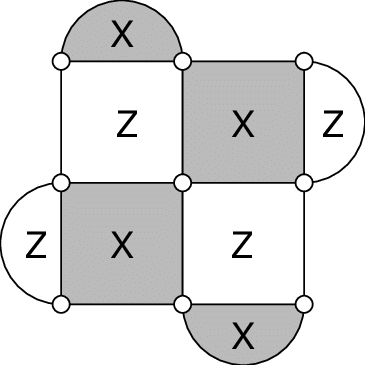
\includegraphics[scale=0.3]{figures/The-smallest-possible-surface-code-consisting-of-9-data-qubits-The-indicated-8.png}
% % \end{figure}

% % \subsubsection{BB Code}
% % \textcite{liang2026selfdualbivariatebicyclecodes} have found all BB codes using less than 160 qubits. The smallest of these, the $[[16, 4, 4]]$-code, is the only option I have considered because otherwise I run into major memory issues.

% % \subsection{Applying Gates to Error-correcting Patches}